\documentclass[10pt]{article}
\usepackage{tikz}
\usetikzlibrary{shapes.misc}
\usepackage[margin=0cm]{geometry}
\pagestyle{empty}
\tikzstyle{every node}=[cross out, draw, red]

\begin{document}

\vspace*{\fill}
\begin{center}
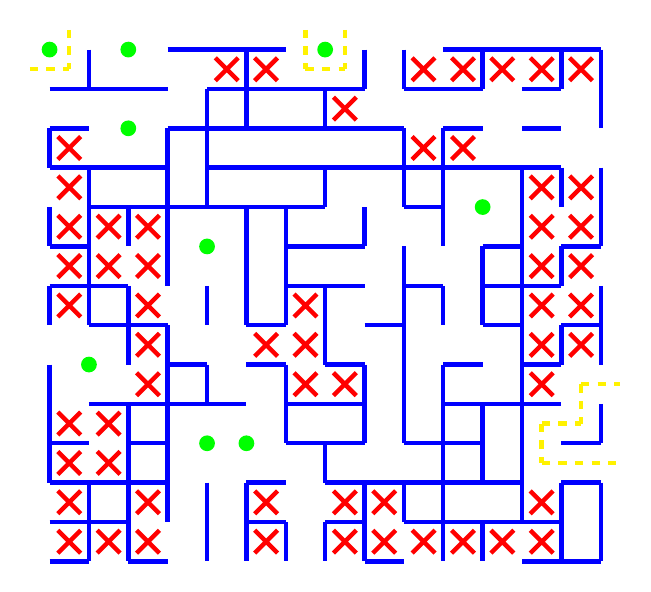
\begin{tikzpicture}[x=0.5cm, y=-0.5cm, ultra thick, blue]
% Walls
    \draw (3,0) -- (6,0);
    \draw (10,0) -- (14,0);
    \draw (0,1) -- (3,1);
    \draw (4,1) -- (8,1);
    \draw (9,1) -- (11,1);
    \draw (12,1) -- (13,1);
    \draw (0,2) -- (1,2);
    \draw (3,2) -- (9,2);
    \draw (10,2) -- (11,2);
    \draw (12,2) -- (13,2);
    \draw (0,3) -- (3,3);
    \draw (4,3) -- (13,3);
    \draw (1,4) -- (7,4);
    \draw (9,4) -- (10,4);
    \draw (0,5) -- (1,5);
    \draw (6,5) -- (8,5);
    \draw (11,5) -- (12,5);
    \draw (13,5) -- (14,5);
    \draw (0,6) -- (2,6);
    \draw (6,6) -- (8,6);
    \draw (9,6) -- (10,6);
    \draw (11,6) -- (13,6);
    \draw (1,7) -- (3,7);
    \draw (5,7) -- (6,7);
    \draw (8,7) -- (9,7);
    \draw (11,7) -- (12,7);
    \draw (13,7) -- (14,7);
    \draw (3,8) -- (4,8);
    \draw (5,8) -- (6,8);
    \draw (7,8) -- (8,8);
    \draw (10,8) -- (11,8);
    \draw (12,8) -- (13,8);
    \draw (1,9) -- (5,9);
    \draw (6,9) -- (8,9);
    \draw (10,9) -- (13,9);
    \draw (0,10) -- (1,10);
    \draw (2,10) -- (3,10);
    \draw (6,10) -- (8,10);
    \draw (9,10) -- (11,10);
    \draw (13,10) -- (14,10);
    \draw (0,11) -- (3,11);
    \draw (5,11) -- (6,11);
    \draw (7,11) -- (12,11);
    \draw (13,11) -- (14,11);
    \draw (0,12) -- (2,12);
    \draw (5,12) -- (6,12);
    \draw (7,12) -- (8,12);
    \draw (9,12) -- (13,12);
    \draw (0,13) -- (1,13);
    \draw (2,13) -- (3,13);
    \draw (8,13) -- (9,13);
    \draw (12,13) -- (14,13);
    \draw (0,2) -- (0,3);
    \draw (0,4) -- (0,5);
    \draw (0,6) -- (0,7);
    \draw (0,8) -- (0,11);
    \draw (1,0) -- (1,1);
    \draw (1,3) -- (1,7);
    \draw (1,11) -- (1,13);
    \draw (2,4) -- (2,5);
    \draw (2,6) -- (2,8);
    \draw (2,9) -- (2,13);
    \draw (3,2) -- (3,6);
    \draw (3,7) -- (3,12);
    \draw (4,1) -- (4,4);
    \draw (4,6) -- (4,7);
    \draw (4,8) -- (4,9);
    \draw (4,11) -- (4,13);
    \draw (5,0) -- (5,2);
    \draw (5,4) -- (5,7);
    \draw (5,11) -- (5,13);
    \draw (6,4) -- (6,7);
    \draw (6,8) -- (6,10);
    \draw (6,12) -- (6,13);
    \draw (7,1) -- (7,2);
    \draw (7,3) -- (7,4);
    \draw (7,6) -- (7,8);
    \draw (7,10) -- (7,11);
    \draw (7,12) -- (7,13);
    \draw (8,0) -- (8,1);
    \draw (8,4) -- (8,5);
    \draw (8,8) -- (8,10);
    \draw (8,11) -- (8,13);
    \draw (9,0) -- (9,1);
    \draw (9,2) -- (9,4);
    \draw (9,5) -- (9,10);
    \draw (9,11) -- (9,12);
    \draw (10,2) -- (10,5);
    \draw (10,6) -- (10,7);
    \draw (10,8) -- (10,13);
    \draw (11,0) -- (11,1);
    \draw (11,5) -- (11,7);
    \draw (11,9) -- (11,11);
    \draw (11,12) -- (11,13);
    \draw (12,3) -- (12,12);
    \draw (13,0) -- (13,1);
    \draw (13,3) -- (13,4);
    \draw (13,5) -- (13,6);
    \draw (13,7) -- (13,8);
    \draw (13,11) -- (13,13);
    \draw (14,0) -- (14,2);
    \draw (14,3) -- (14,5);
    \draw (14,6) -- (14,8);
    \draw (14,9) -- (14,10);
    \draw (14,11) -- (14,13);
% Pillars
    \fill[green] (0,0) circle(0.2);
    \fill[green] (2,0) circle(0.2);
    \fill[green] (7,0) circle(0.2);
    \fill[green] (2,2) circle(0.2);
    \fill[green] (11,4) circle(0.2);
    \fill[green] (4,5) circle(0.2);
    \fill[green] (1,8) circle(0.2);
    \fill[green] (4,10) circle(0.2);
    \fill[green] (5,10) circle(0.2);
% Inner points in accessible cul-de-sacs
    \node at (4.5,0.5) {};
    \node at (5.5,0.5) {};
    \node at (9.5,0.5) {};
    \node at (10.5,0.5) {};
    \node at (11.5,0.5) {};
    \node at (12.5,0.5) {};
    \node at (13.5,0.5) {};
    \node at (7.5,1.5) {};
    \node at (0.5,2.5) {};
    \node at (9.5,2.5) {};
    \node at (10.5,2.5) {};
    \node at (0.5,3.5) {};
    \node at (12.5,3.5) {};
    \node at (13.5,3.5) {};
    \node at (0.5,4.5) {};
    \node at (1.5,4.5) {};
    \node at (2.5,4.5) {};
    \node at (12.5,4.5) {};
    \node at (13.5,4.5) {};
    \node at (0.5,5.5) {};
    \node at (1.5,5.5) {};
    \node at (2.5,5.5) {};
    \node at (12.5,5.5) {};
    \node at (13.5,5.5) {};
    \node at (0.5,6.5) {};
    \node at (2.5,6.5) {};
    \node at (6.5,6.5) {};
    \node at (12.5,6.5) {};
    \node at (13.5,6.5) {};
    \node at (2.5,7.5) {};
    \node at (5.5,7.5) {};
    \node at (6.5,7.5) {};
    \node at (12.5,7.5) {};
    \node at (13.5,7.5) {};
    \node at (2.5,8.5) {};
    \node at (6.5,8.5) {};
    \node at (7.5,8.5) {};
    \node at (12.5,8.5) {};
    \node at (0.5,9.5) {};
    \node at (1.5,9.5) {};
    \node at (0.5,10.5) {};
    \node at (1.5,10.5) {};
    \node at (0.5,11.5) {};
    \node at (2.5,11.5) {};
    \node at (5.5,11.5) {};
    \node at (7.5,11.5) {};
    \node at (8.5,11.5) {};
    \node at (12.5,11.5) {};
    \node at (0.5,12.5) {};
    \node at (1.5,12.5) {};
    \node at (2.5,12.5) {};
    \node at (5.5,12.5) {};
    \node at (7.5,12.5) {};
    \node at (8.5,12.5) {};
    \node at (9.5,12.5) {};
    \node at (10.5,12.5) {};
    \node at (11.5,12.5) {};
    \node at (12.5,12.5) {};
% Entry-exit paths without intersections
    \draw[dashed, yellow] (-0.5,0.5) -- (0.5,0.5);
    \draw[dashed, yellow] (6.5,0.5) -- (7.5,0.5);
    \draw[dashed, yellow] (13.5,8.5) -- (14.5,8.5);
    \draw[dashed, yellow] (12.5,9.5) -- (13.5,9.5);
    \draw[dashed, yellow] (12.5,10.5) -- (14.5,10.5);
    \draw[dashed, yellow] (0.5,-0.5) -- (0.5,0.5);
    \draw[dashed, yellow] (6.5,-0.5) -- (6.5,0.5);
    \draw[dashed, yellow] (7.5,-0.5) -- (7.5,0.5);
    \draw[dashed, yellow] (12.5,9.5) -- (12.5,10.5);
    \draw[dashed, yellow] (13.5,8.5) -- (13.5,9.5);
\end{tikzpicture}
\end{center}
\vspace*{\fill}

\end{document}
